\section{Additional Results}
\label{app:additional-results}

\paragraph{Coverage Desiderata.}
\label{app:sequence-metrics-full}
% Generated by assets/tables/make_sequence_metrics_goldsim_table.py — do not edit by hand.
\begin{table}[H]
\centering
\caption{Sequence-level diagnostics. \emph{Gold} columns score the action lists in each task's evaluation criteria. \emph{GoldSim} columns score one representative agent sequence per task, selected as the shortest run with $\texttt{db\_reward}\!=\!1$ across all in-scope simulations; tasks with no successful run fall back to the gold action list. Selection rule and aggregation are detailed in Section~\ref{app:sequence-metrics-full}.}
\label{tab:sequence-metrics-goldsim}
\scriptsize
\setlength{\tabcolsep}{3pt}
\renewcommand{\arraystretch}{0.85}
\vspace{1mm}
\begin{tabular}{l cccc @{\hspace{0.6em}} cccc @{\hspace{0.6em}} cccc}
\toprule
 & \multicolumn{4}{c}{Airline} & \multicolumn{4}{c}{Retail} & \multicolumn{4}{c}{Telecom} \\
\cmidrule(lr){2-5}\cmidrule(lr){6-9}\cmidrule(lr){10-13}
 & \multicolumn{2}{c}{Gold} & \multicolumn{2}{c}{GoldSim} & \multicolumn{2}{c}{Gold} & \multicolumn{2}{c}{GoldSim} & \multicolumn{2}{c}{Gold} & \multicolumn{2}{c}{GoldSim} \\
\cmidrule(lr){2-3}\cmidrule(lr){4-5}\cmidrule(lr){6-7}\cmidrule(lr){8-9}\cmidrule(lr){10-11}\cmidrule(lr){12-13}
Metric & TBV & \textbf{Ours} & TBV & \textbf{Ours} & TBV & \textbf{Ours} & TBV & \textbf{Ours} & TBV & \textbf{Ours} & TBV & \textbf{Ours} \\
\midrule
\rowcolor[gray]{0.95}
Avg.\ length & 2.84 & 11.36 & 4.68 & 10.64 & 4.82 & 10.66 & 6.58 & 9.19 & 4.53 & 6.50 & 6.60 & 7.64 \\
W/R ratio & 0.53 & 0.31 & 0.27 & 0.37 & 0.47 & 0.32 & 0.30 & 0.40 & {--} & {--} & 0.35 & 0.68 \\
\rowcolor[gray]{0.95}
WED intra & 3.76 & 8.42 & 5.20 & 8.34 & 4.89 & 7.07 & 4.18 & 6.70 & 4.32 & 5.50 & 6.63 & 7.05 \\
\rowcolor[gray]{0.95}
Entropy 1-gram & 2.60 & 3.50 & 2.80 & 3.51 & 3.23 & 3.38 & 3.01 & 3.38 & 3.86 & 4.34 & 4.61 & 4.80 \\
Entropy 2-gram & 3.42 & 6.68 & 4.12 & 6.54 & 4.64 & 6.22 & 4.27 & 6.02 & 5.17 & 7.67 & 6.44 & 8.10 \\
\rowcolor[gray]{0.95}
Entropy 3-gram & 3.69 & 8.22 & 4.65 & 8.18 & 5.29 & 8.24 & 5.14 & 7.94 & 5.90 & 8.33 & 7.29 & 8.78 \\
Entropy 4-gram & 3.63 & 8.58 & 4.73 & 8.50 & 5.87 & 9.27 & 5.90 & 8.84 & 6.05 & 8.20 & 7.60 & 8.73 \\
\rowcolor[gray]{0.95}
Entropy 1-gram (norm.) & 0.68 & 0.92 & 0.74 & 0.92 & 0.83 & 0.86 & 0.77 & 0.86 & 0.71 & 0.80 & 0.85 & 0.88 \\
Entropy 2-gram (norm.) & 0.45 & 0.88 & 0.54 & 0.86 & 0.59 & 0.80 & 0.55 & 0.77 & 0.48 & 0.71 & 0.59 & 0.75 \\
\rowcolor[gray]{0.95}
Entropy 3-gram (norm.) & 0.32 & 0.72 & 0.41 & 0.72 & 0.45 & 0.70 & 0.44 & 0.68 & 0.36 & 0.51 & 0.45 & 0.54 \\
Entropy 4-gram (norm.) & 0.24 & 0.56 & 0.31 & 0.56 & 0.38 & 0.59 & 0.38 & 0.57 & 0.28 & 0.38 & 0.35 & 0.40 \\
\rowcolor[gray]{0.95}
Entropy avg.\ (norm.) & 0.42 & 0.77 & 0.50 & 0.76 & 0.56 & 0.74 & 0.53 & 0.72 & 0.46 & 0.60 & 0.56 & 0.64 \\
\# unique seqs & 30 & 50 & 40 & 50 & 75 & 114 & 94 & 112 & 94 & 114 & 107 & 102 \\
\rowcolor[gray]{0.95}
\# unique 2-gram & 20 & 133 & 41 & 135 & 65 & 127 & 64 & 132 & 57 & 279 & 149 & 374 \\
\# unique 3-gram & 24 & 333 & 56 & 322 & 92 & 418 & 108 & 386 & 86 & 365 & 228 & 494 \\
\rowcolor[gray]{0.95}
\# unique 4-gram & 23 & 393 & 54 & 368 & 105 & 680 & 130 & 560 & 93 & 317 & 255 & 451 \\
\# unique 5-gram & 18 & 362 & 47 & 334 & 103 & 725 & 139 & 552 & 80 & 244 & 234 & 371 \\
\rowcolor[gray]{0.95}
\# unique 6-gram & 14 & 315 & 42 & 288 & 86 & 644 & 135 & 491 & 60 & 171 & 200 & 288 \\
TTR 2-gram & 0.20 & 0.26 & 0.22 & 0.28 & 0.15 & 0.12 & 0.10 & 0.14 & 0.14 & 0.44 & 0.23 & 0.49 \\
\rowcolor[gray]{0.95}
TTR 3-gram & 0.32 & 0.71 & 0.38 & 0.74 & 0.27 & 0.42 & 0.21 & 0.47 & 0.28 & 0.71 & 0.43 & 0.77 \\
TTR 4-gram & 0.42 & 0.94 & 0.46 & 0.96 & 0.39 & 0.78 & 0.31 & 0.79 & 0.41 & 0.78 & 0.61 & 0.84 \\
\rowcolor[gray]{0.95}
TTR 5-gram & 0.44 & 0.98 & 0.51 & 1.00 & 0.51 & 0.96 & 0.44 & 0.92 & 0.49 & 0.80 & 0.71 & 0.86 \\
TTR 6-gram & 0.47 & 0.99 & 0.55 & 1.00 & 0.61 & 0.99 & 0.60 & 0.98 & 0.56 & 0.81 & 0.78 & 0.88 \\
\rowcolor[gray]{0.95}
\# unique avg.\ (TTR) & 0.37 & 0.78 & 0.43 & 0.80 & 0.39 & 0.65 & 0.33 & 0.66 & 0.38 & 0.71 & 0.55 & 0.77 \\
\bottomrule
\end{tabular}
\end{table}





Table~\ref{tab:sequence-metrics-goldsim} extends the results presented in Figure~\ref{fig:coverage_fig} to the full set of sequence-level statistics: average length (mean number of tool calls per sequence); write/read balance (ratio of write tools to read and generic tools); within-cluster weighted edit distance (\emph{WED intra} - mean pairwise distance over all sequence pairs in the cluster, indicating intra-set diversity); Shannon entropy at \mbox{$n=1\ldots4$} (n-gram occurrences are tallied with a sliding window, normalised to a probability distribution, then $H_n=-\sum_g p(g)\log_2 p(g)$) together with their vocabulary-normalised mean ($H_n/(n\log_2|V|)$ averaged   over $n$, in $[0,1]$, allowing comparison across cells with different tool vocabularies); the count of unique $n$-grams at $n=2\ldots6$ (compositional richness); and the mean type-token ratio (unique $n$-grams divided by total $n$-grams positions, averaged over $n=2\ldots6$; higher means less repetition). The reported numbers compare against \emph{GoldSim}; how we extract it is explained in the following paragraph.

\paragraph{The GoldSim simulation set.}
The \emph{GoldSim} columns aggregate agent behaviour into one representative tool sequence per task. Concretely, for a given (domain, task-set) cell we proceed as follows:
\begin{enumerate}
    \item \textbf{Run pool.} For every task $i$, gather the union of all simulation runs, pooled across agent, user simulator, and trial $k$. Filter unsuccessful runs (reward$=0.0$).
    \item \textbf{Sequence extraction.} For each run we read the agent's tool calls in turn order and concatenate their identifiers into one ordered tool sequence ($\bar\sigma$).
    \item \textbf{Per-task pick.} If more then a single candidate exist, we pick the candidate of \emph{minimal length}. The intuition is that the shortest successful trajectory is the cleanest evidence of a working solution path.
    \item \textbf{Gold fallback.} If no candidate exists for task $i$ ---  we use the task's gold tool sequence ($\bar\sigma^\star$). This keeps the per-cell sequence count equal to the cell's task count and avoids selection bias against hard tasks.
\end{enumerate}

\paragraph{Difficulty Desiderata.}
\label{app:difficulty-desiderata}
\begin{figure}[H]
    \centering
    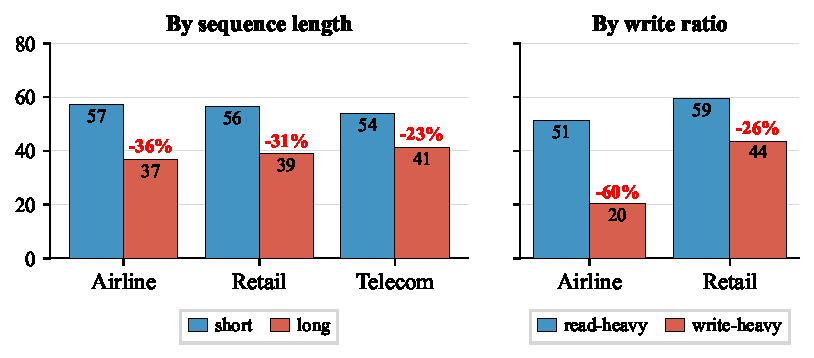
\includegraphics[width=0.7\linewidth]{assets/figures/difficulty_desiderata/difficulty_desiderata.pdf}
    \caption{Mean accuracy on tasks bucketed by per-task golden-sequence length (left) and write-ratio (right), using $\mu \pm 0.5\sigma$ thresholds with the middle band dropped.}
    \label{fig:difficulty-desiderata}
\end{figure}

Figure~\ref{fig:difficulty-desiderata} validates the two structural axes we use to control task difficulty. Splitting tasks by per-task golden-sequence length produces a $13$--$20$\,pp accuracy gap between short and long buckets across all three domains. Splitting by per-task write-ratio produces a $16$--$31$\,pp gap between read-heavy and write-heavy buckets in airline and retail. Telecom is excluded from the write-ratio panel because its evaluation criteria encode only write actions, so per-task write-ratio collapses to $1.0$ for every task. These results indicate that compositional length and write-heaviness act as genuine difficulty knobs rather than descriptive labels, supporting their use as control axes when sampling harder tasks.

\paragraph{Tool-Usage Distributions Across Domains.}
\label{app:tool-use-dist}
Figure~\ref{fig:diversity-combined} reports complementary diversity views across the three \taubench domains. Each plot the per-tool relative frequency of the \tbv\xspace against \ourbenchmark; the latter spreads usage more evenly across the tool vocabulary, raising the normalised entropy ($H$ = Shannon entropy / $\log_2 |\text{tools}|$) reported in each legend.
% Combined diversity diagnostic figure for the appendix.
% Replaces the two separate figures (ngram_ttr_domains_tex,
% tool_diversity_appendix_tex) with one figure that has subfigures (a)/(b).
\begin{figure}[H]
\centering

\begin{minipage}[t]{0.49\linewidth}
    \centering
    \vspace*{0pt}%
    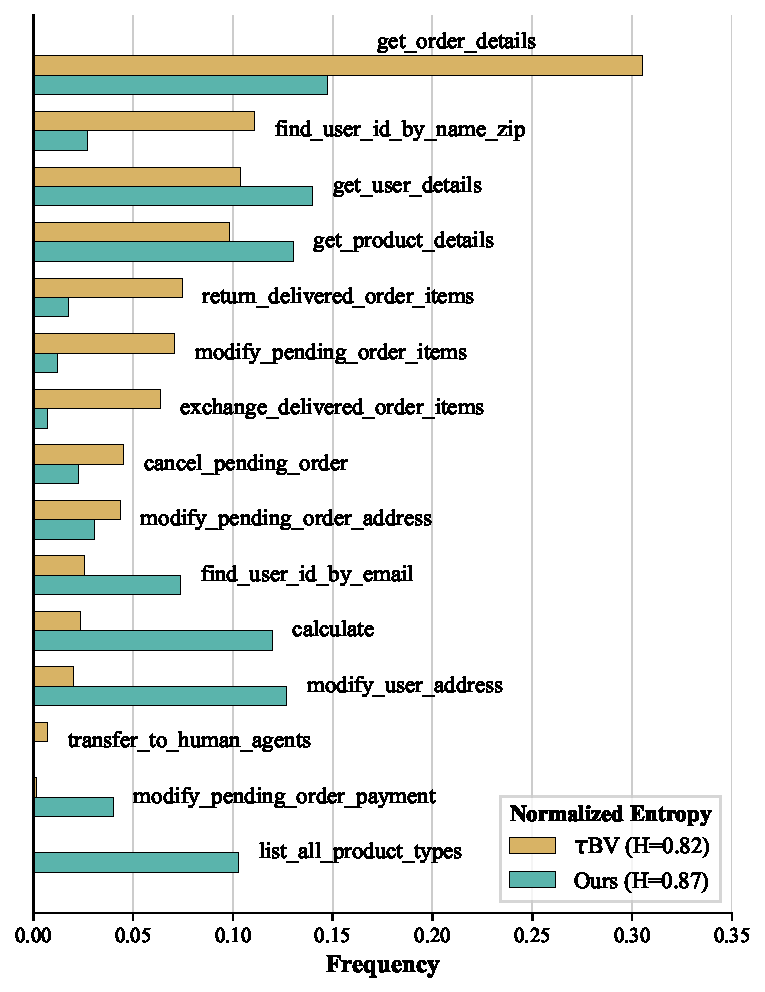
\includegraphics[width=\linewidth]{assets/figures/tool_frequency_retail.pdf}\\
    \textbf{(a) retail}
\end{minipage}%
\hfill
\begin{minipage}[t]{0.49\linewidth}
    \centering
    \vspace*{0pt}%
    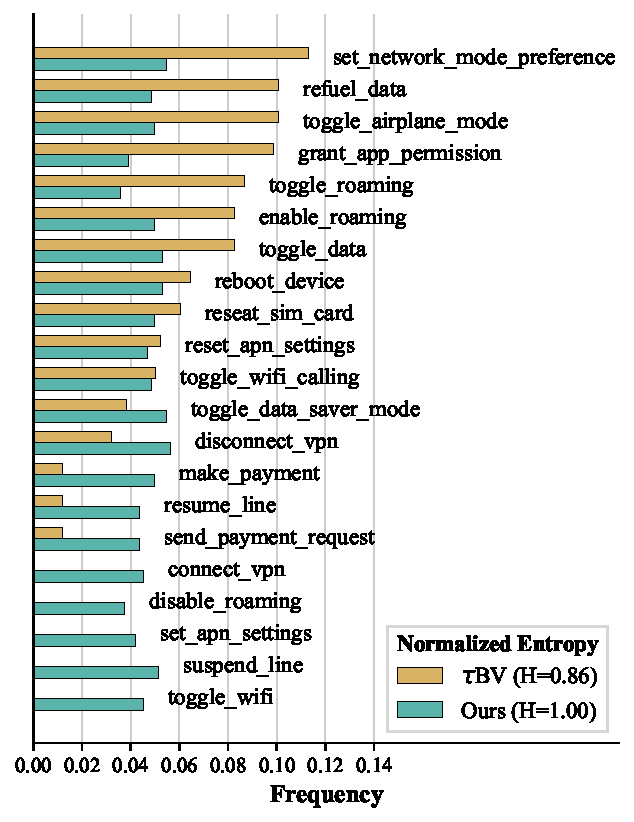
\includegraphics[width=\linewidth]{assets/figures/tool_frequency_telecom.pdf}\\
    \textbf{(b) telecom (write actions only)}
\end{minipage}

\caption{Per-tool relative frequency on the retail and telecom domains, comparing \tbv\xspace against \ourbenchmark; the airline counterpart is in Figure~\ref{fig:coverage_fig}. Normalised entropy $H$ is reported in each panel's legend; tools are ordered within each panel by \tbv\xspace task frequency. Telecom is restricted to write actions (21 of 43 tools, both distributions re-normalised over this subset) since the \tbv\xspace telecom tasks does not include read tools in their gold tool sequences.}
\label{fig:diversity-combined}
\end{figure}


\paragraph{Qualitative Comparison: Weighted vs.\ Regular Edit Distance.}
\label{app:wed-qualitative}
Figure~\ref{fig:cluster-distances} (Appendix~\ref{app:examples}) contrasts $k$-medoids clustering on airline trajectories under our weighted edit distance (WED) and the unweighted edit distance (ED). Under WED \textbf{(a)}, the three medoids correspond to clear, distinct user-service intents -- \emph{search/book/update}, \emph{demand a refund}, and \emph{book and update} -- and each medoid's nearest neighbors stay close to it semantically: they share the medoid's overall intent and only differ in surface-level details. Under ED \textbf{(b)}, the medoids themselves remain interpretable, but the nearest neighbors drift away from the medoid's intent, mixing in unrelated tool subsequences. Figure \textbf{(c)} makes the same point quantitatively: under WED the inter-medoid distances ($3.66$--$4.66$) are larger than the intra-cluster neighbor distances visible, whereas under ED inter- and intra-cluster scales are closer, reflecting weaker cluster separation. Together, these examples illustrate why we use WED rather than plain edit distance for the clustering step in Section~\ref{sub:clustering}: the type-aware substitution costs translate into clusters whose members are semantically coherent, not just superficially similar.
